\setcounter{page}{2}

\subsection*{Структура FILE}
\begin{center}
	\captionsetup{justification=raggedright,singlelinecheck=off}

	\begin{lstlisting}[label=lst:file-1,caption=Структура FILE, часть 1]
		typedef struct _IO_FILE FILE;
struct _IO_FILE
{
  int _flags;		/* High-order word is _IO_MAGIC; rest is flags. */

  /* The following pointers correspond to the C++ streambuf protocol. */
  char *_IO_read_ptr;	/* Current read pointer */
  char *_IO_read_end;	/* End of get area. */
  char *_IO_read_base;	/* Start of putback+get area. */
  char *_IO_write_base;	/* Start of put area. */
  char *_IO_write_ptr;	/* Current put pointer. */
  char *_IO_write_end;	/* End of put area. */
  char *_IO_buf_base;	/* Start of reserve area. */
  char *_IO_buf_end;	/* End of reserve area. */

/* The following fields are used to support backing up and undo. */
  char *_IO_save_base; /* Pointer to start of non-current get area. */
  char *_IO_backup_base;  /* Pointer to first valid character of backup area */
  char *_IO_save_end; /* Pointer to end of non-current get area. */

  struct _IO_marker *_markers;

  struct _IO_FILE *_chain;

  int _fileno;
  int _flags2;
  __off_t _old_offset; /* This used to be _offset but it's too small.  */
	\end{lstlisting}
\end{center}

\clearpage

\begin{center}
	\captionsetup{justification=raggedright,singlelinecheck=off}

	\begin{lstlisting}[label=lst:file-2,caption=Структура FILE, часть 2]
/* 1+column number of pbase(); 0 is unknown. */
  unsigned short _cur_column;
  signed char _vtable_offset;
  char _shortbuf[1];

  _IO_lock_t *_lock;
  #ifdef _IO_USE_OLD_IO_FILE
};
	\end{lstlisting}
\end{center}

\subsection*{Программа 1, один поток}

\begin{center}
	\captionsetup{justification=raggedright,singlelinecheck=off}

	\begin{lstlisting}[label=lst:prog1-1,caption=Программа 1 --- один поток--- часть 1]
#include <stdio.h>
#include <fcntl.h>

int main()
{
    int fd = open("alphabet.txt", O_RDONLY);

    FILE *fs1 = fdopen(fd,"r");
    char buff1[20];
    setvbuf(fs1,buff1,_IOFBF,20);

    FILE *fs2 = fdopen(fd,"r");
    char buff2[20];
    setvbuf(fs2,buff2,_IOFBF,20);
    
    int flag1 = 1, flag2 = 1;
    while(flag1 == 1 || flag2 == 1)
    {
        char c;
        flag1 = fscanf(fs1,"%c",&c);
        if (flag1 == 1) 
        {
            fprintf(stdout,"%c",c);
        }
        flag2 = fscanf(fs2,"%c",&c);
	\end{lstlisting}
\end{center}

\clearpage

\begin{center}
	\captionsetup{justification=raggedright,singlelinecheck=off}

	\begin{lstlisting}[label=lst:prog1-2,caption=Программа 1 --- один поток --- часть 2]
        if (flag2 == 1) 
        { 
            fprintf(stdout,"%c",c); 
        }
    }
    printf("\n");
    return 0;
}
	\end{lstlisting}
\end{center}

Результаты работы:

\begin{figure}[h]
	\centering
	\captionsetup{justification=centering}
	
\includegraphics[width=150mm]{img/prog1.png}
	\caption{Результаты работы программы 1 (один поток)}
	\label{fig:prog-1-result}
\end{figure}

\subsection*{Программа 1, два потока}


\begin{center}
	\captionsetup{justification=raggedright,singlelinecheck=off}

	\begin{lstlisting}[label=lst:prog1-th-1,caption=Программа 1 --- два потока --- часть 1]
#include <fcntl.h>
#include <pthread.h>
#include <stdio.h>

void *thread_routine(void *fd) 
{
    int flag = 1;
    char c;

    FILE *fs = fdopen(*((int *)fd), "r");
    char buf[20];
    setvbuf(fs, buf, _IOFBF, 20);

    while (flag == 1) 
    {
        flag = fscanf(fs, "%c", &c);
        if (flag == 1) 
        {
            fprintf(stdout, "%c", c);
        }
	\end{lstlisting}
\end{center}

\clearpage

\begin{center}
	\captionsetup{justification=raggedright,singlelinecheck=off}

	\begin{lstlisting}[label=lst:prog1-th-2,caption=Программа 1 --- два потока --- часть 2]
    }
}

int main(void) 
{
    int fd = open("alphabet.txt", O_RDONLY);

    FILE *fs = fdopen(fd, "r");
    char buf[20];
    setvbuf(fs, buf, _IOFBF, 20);

    pthread_t thr_worker;

    pthread_create(&thr_worker, NULL, thread_routine, &fd);

    int flag = 1;
    char c;
    while (flag == 1) 
    {
        flag = fscanf(fs, "%c", &c);
        if (flag == 1) 
        {
            fprintf(stdout, "%c", c);
        }
    }
    pthread_join(thr_worker, NULL);
    printf("\n");
    return 0;
}
	\end{lstlisting}
\end{center}

Результаты работы:

\begin{figure}[h]
	\centering
	\captionsetup{justification=centering}
	
\includegraphics[width=150mm]{img/prog1_thread.png}
	\caption{Результаты работы программы 1 (два потока)}
	\label{fig:prog-1-th-result}
\end{figure}

\subsubsection*{Анализ полученного результата}

Системный вызов $open$ возвращает дескриптор $fd$ типа $int$ открытого файла, затем два раза вызывается $fdopen$, которой передаётся полученный дескриптор $fd$. Функция возвращает указатель на структуру $FILE$.

Функция $setvbuf$ задаёт размер буфера 20 байт, создаются два буфера.

%Функции $fscanf(fs1, "\%c", \&c)$ копирует в буфер $buff1$ первые 20 символов (т.е. $abcdefghijklmnopqrst$), в переменную $c$ записывается ) буква $a$. 
%
%$fscanf(fs2, "\%c", \&c)$ копирует в буфер $buff2$ оставшиеся символы (т.е. $uvwxyz$), в переменную $c$ записывается буква $u$.

%В цикле будут поочерёдно выводиться символы из буферов $buff1$ и $buff2$ до тех пор, пока символы в одном из них не закончатся.
%После этого будут выведены оставшиеся символы из другого буфера.

Предполагается, что, читая в цикле сначала по указателю fs1, а потом по указателю fs2, можно предположить, что символы будут прочитаны последовательно, однако буферизованный ввод-вывод приводит к тому, что при первом вызове заполняется буфер (т.е. 20 символов), которые будут выведены на экран.

При втором вызове заполняется второй буфер оставшимися символами (до символа окончания файла), и затем они выводятся на экран.

Таким образом, полученный результат является следствием буферизации,

\subsubsection*{Связь структур}


\begin{figure}[h]
	\centering
	\captionsetup{justification=centering}
	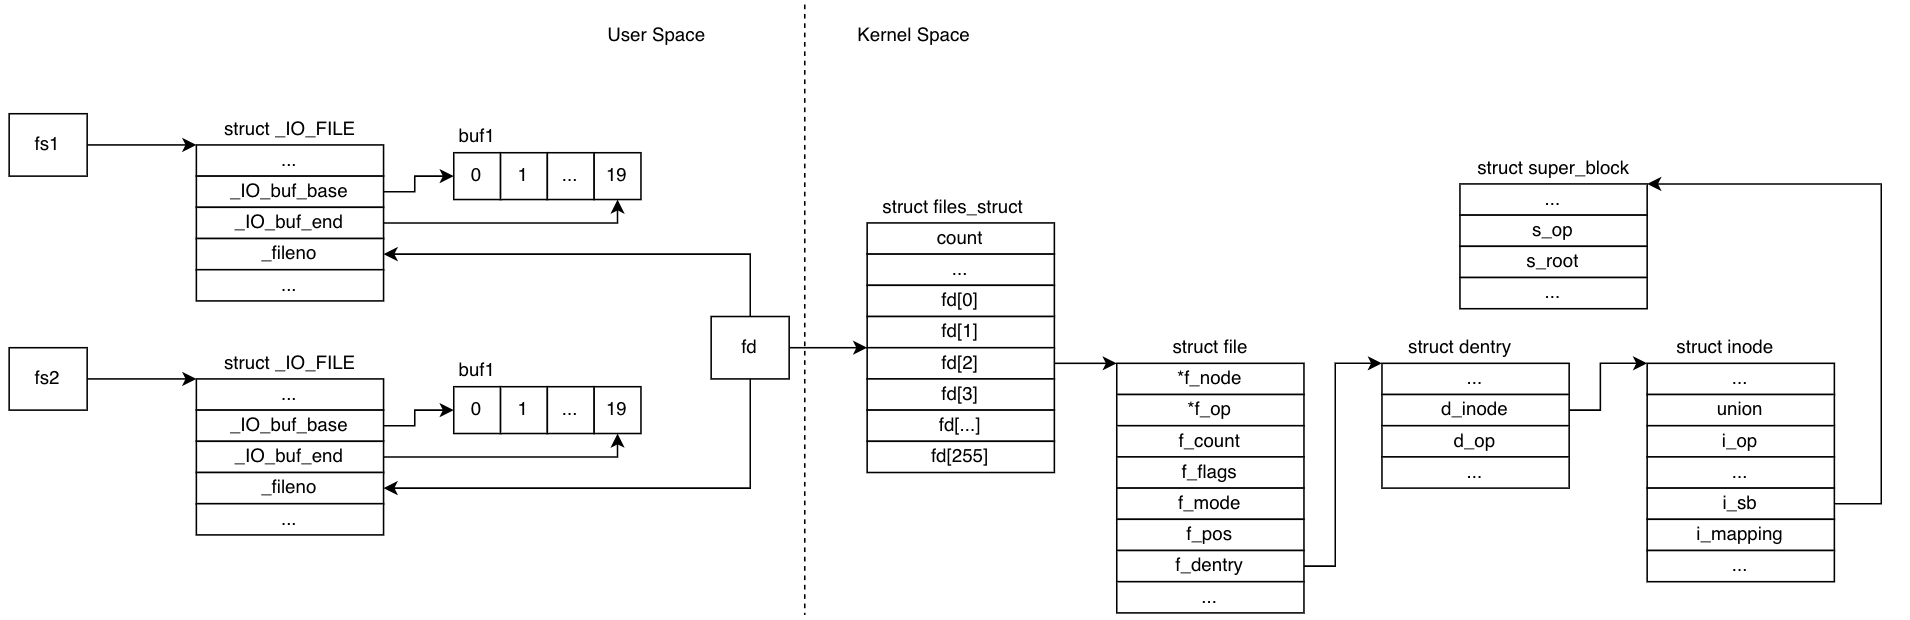
\includegraphics[width=160mm]{img/prog1_diagram.png}
	\caption{Связь структур}
	\label{fig:prog-1-diagram}
\end{figure}

\clearpage

\subsection*{Программа 2, один поток}

\begin{center}
	\captionsetup{justification=raggedright,singlelinecheck=off}

	\begin{lstlisting}[label=lst:prog2,caption=Программа 2 --- один поток]
#include <stdio.h>
#include <fcntl.h>
#include <unistd.h>

int main()
{
    char c;    
    int fd1 = open("alphabet.txt", O_RDONLY);
    int fd2 = open("alphabet.txt", O_RDONLY);

    int flag1 = 1, flag2 = 1;
    while(flag1 == 1 || flag2 == 1)
    {
        char c;
        flag1 = read(fd1,&c,1);
        if (flag1 == 1) 
        {
            write(1,&c,1);
        }
        flag2 = read(fd2,&c,1);
        if (flag2 == 1) 
        { 
            write(1,&c,1);
        }
    }
    printf("\n");
    return 0;
}
	\end{lstlisting}
\end{center}

Результаты работы:

\begin{figure}[h]
	\centering
	\captionsetup{justification=centering}
	
\includegraphics[width=150mm]{img/prog2.png}
	\caption{Результаты работы программы 2 (один поток)}
	\label{fig:prog-2-result}
\end{figure}

\clearpage

\subsection*{Программа 2, два потока}

\begin{center}
	\captionsetup{justification=raggedright,singlelinecheck=off}

	\begin{lstlisting}[label=lst:prog2-th-1,caption=Программа 2 --- два потока --- часть 1]
#include <fcntl.h>
#include <pthread.h>
#include <stdio.h>
#include <unistd.h>

void *thread_routine(void *arg)
{
    int fd = *((int *)arg);

    int flag = 1;
    char c;

    while (flag == 1)
    {
        flag = read(fd, &c, 1);
        if (flag == 1)
            write(1, &c, 1);
    }
}

int main()
{
    int fd1 = open("alphabet.txt", O_RDONLY);
    int fd2 = open("alphabet.txt", O_RDONLY);

    pthread_t thr_worker;

    pthread_create(&thr_worker, NULL, thread_routine, &fd1);

    int flag = 1;
    char c;
    while (flag == 1)
    {
        flag = read(fd2, &c, 1);
        if (flag == 1)
            write(1, &c, 1);
    }
	\end{lstlisting}
\end{center}

\clearpage

\begin{center}
	\captionsetup{justification=raggedright,singlelinecheck=off}

	\begin{lstlisting}[label=lst:prog2-th-2,caption=Программа 2 --- два потока --- часть 2]
    pthread_join(thr_worker, NULL);
    printf("\n");
    return 0;
}
	\end{lstlisting}
\end{center}

Результаты работы:

\begin{figure}[h]
	\centering
	\captionsetup{justification=centering}
	
\includegraphics[width=150mm]{img/prog2_thread.png}
	\caption{Результаты работы программы 2 (два потока)}
	\label{fig:prog-2-th-result}
\end{figure}

\subsubsection*{Анализ результата}

Системные вызовы $open$ для открытия файла $alphabet.txt$ создают дескрипторы $fs1$ и $fs2$  типа $int$ открытых файлов и создают структуры $struct file$.

Поочерёдный вызов $read$ для  $fs1$ и $fs2$ меняет значения полей $f\_pos$ в структурах $struct file$, что приводит к полному прочтению $alphabet.txt$ 2 раза.


\clearpage

\subsubsection*{Связь структур}

\begin{figure}[h]
	\centering
	\captionsetup{justification=centering}
	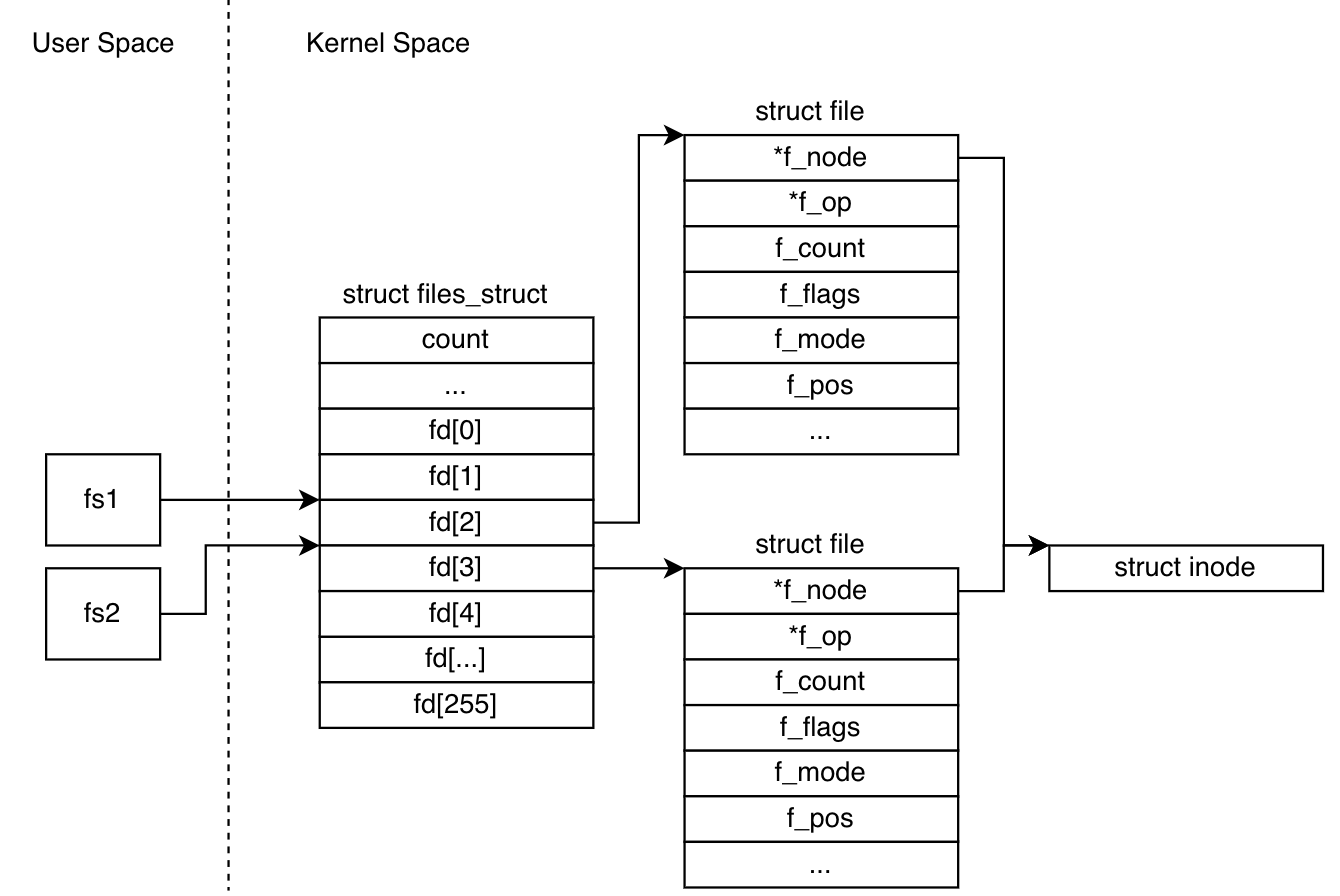
\includegraphics[width=160mm]{img/prog2_diagram.png}
	\caption{Связь структур}
	\label{fig:prog-2-diagram}
\end{figure}

\subsection*{Программа 3, один поток}

\begin{center}
	\captionsetup{justification=raggedright,singlelinecheck=off}

	\begin{lstlisting}[label=lst:prog3-1,caption=Программа 3 --- один поток --- часть 1]
#include <fcntl.h>
#include <stdio.h>
#include <unistd.h>

int main() 
{
    FILE *f1 = fopen("out.txt", "w");
    FILE *f2 = fopen("out.txt", "w");

    for (char letr = 'a'; letr < '{'; letr++) 
    {
        letr % 2 ? fprintf(f1, "%c", letr) : fprintf(f2, "%c", letr);
    }
	\end{lstlisting}
\end{center}

\clearpage

\begin{center}
	\captionsetup{justification=raggedright,singlelinecheck=off}

	\begin{lstlisting}[label=lst:prog3-2,caption=Программа 3 --- один поток --- часть 2]
    fprintf(f1, "\n");
    fclose(f2);
    fclose(f1);
    return 0;
}
	\end{lstlisting}
\end{center}

Результаты работы:

\begin{figure}[h]
	\centering
	\captionsetup{justification=centering}
	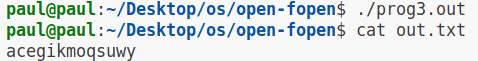
\includegraphics[width=150mm]{img/prog3.png}
	\caption{Результаты работы программы 3 (один поток)}
	\label{fig:prog-3-result}
\end{figure}

\subsection*{Программа 3, два потока}

\begin{center}
	\captionsetup{justification=raggedright,singlelinecheck=off}

	\begin{lstlisting}[label=lst:prog3-th-1,caption=Программа 3 --- два потока --- часть 1]
#include <fcntl.h>
#include <pthread.h>
#include <stdio.h>
#include <sys/stat.h>
#include <unistd.h>

struct stat statbuf;

void *thread_routine() 
{
    FILE *f2 = fopen("out.txt", "a");
    stat("out.txt", &statbuf);
    printf("open for fs2: inode  = %ld, buffsize = %ld blocksize= %ld\n",
        (long int)statbuf.st_ino, (long int)statbuf.st_size,
        (long int)statbuf.st_blksize);

    for (char letr = 'a'; letr < '{'; letr += 2) 
        fprintf(f2, "%c", letr);
    fclose(f2);
    stat("out.txt", &statbuf);
	\end{lstlisting}
\end{center}

\clearpage

\begin{center}
	\captionsetup{justification=raggedright,singlelinecheck=off}

	\begin{lstlisting}[label=lst:prog3-th-2,caption=Программа 3 --- два потока --- часть 2]
    printf("close for fs2: inode  = %ld, buffsize = %ld blocksize= %ld\n",
        (long int)statbuf.st_ino, (long int)statbuf.st_size,
        (long int)statbuf.st_blksize);
}

int main() 
{
    FILE *f1 = fopen("out.txt", "a");
    stat("out.txt", &statbuf);
    printf("open for fs1: inode  = %ld, buffsize = %ld blocksize= %ld\n",
        (long int)statbuf.st_ino, (long int)statbuf.st_size,
        (long int)statbuf.st_blksize);
    pthread_t thr_worker;
    pthread_create(&thr_worker, NULL, thread_routine, f1);
    pthread_join(thr_worker, NULL);

    for (char letr = 'a'; letr < '{'; letr += 2) 
        fprintf(f1, "%c", letr);

    fprintf(f1, "\n");
    fclose(f1);
    stat("out.txt", &statbuf);
    printf("close for fs2: inode  = %ld, buffsize = %ld blocksize= %ld\n",
        (long int)statbuf.st_ino, (long int)statbuf.st_size,
        (long int)statbuf.st_blksize);

    return 0;
}
	\end{lstlisting}
\end{center}

\clearpage

Результаты работы:

\begin{figure}[h]
	\centering
	\captionsetup{justification=centering}
	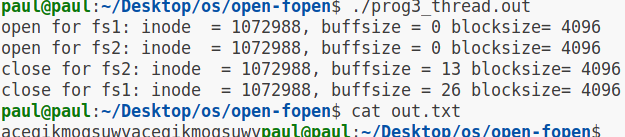
\includegraphics[width=150mm]{img/prog3_thread.png}
	\caption{Результаты работы программы 3 (один поток)}
	\label{fig:prog-3-th-result}
\end{figure}

\subsubsection*{Анализ результатов}

Системные вызовы $open$ для открытия файла $alphabet.txt$ создают дескрипторы $fs1$ и $fs2$  открытых файлов и создают структуры $struct file$.

Поочерёдный вызов $read$ для  $fs1$ и $fs2$ меняет значения полей $f\_pos$ в структурах $struct file$, что приводит к полному прочтению $alphabet.txt$ 2 раза.

Вызовы $fopen$ открытия файла $out.txt$ производят системный вызовы $open$, которые открывают файл $out.txt$ и создают структуры $struct file$.

Функция $fprintf$ получает указатель на буфер, в который информация помещается перед тем, как быть записана в файл.

Из буфера информация копируется в файл при выполнении одного из трёх условий:

\begin{enumerate}
	\item Буфер заполнен.
	\item Вызван $fflush$ для принудительной записи в файл.
	\item Вызван $fclose$.
\end{enumerate}

Проблемой такого использования fprintf является утеря данных: в файле оказывается только содержимое буфера $f2$, поскольку запись происходит в следующем порядке: сначала при вызове $fclose$ для $f1$ (буфер $f1$ записывается в файл), после чего при вызове $fclose$ для $f2$ (буфер $f2$ записывается в файл).

Данную проблему можно решить, используя флаг $O\_APPEND$ при вызове функции $open$ --- это гарантирует добавление данных в конец файла.
Также можно использовать средства взаимоисключения, такие, как $mutex$-ы и семафоры.

\clearpage

\subsection*{Программа 3, open и O\_APPEND}
\begin{center}
	\captionsetup{justification=raggedright,singlelinecheck=off}

\begin{lstlisting}[label=lst:prog3-th-2,caption=Программа 3 --- open]
#include <stdio.h>
#include <fcntl.h>
#include <unistd.h>

int main()
{
    char *alphabet = "abcdefghijklmnopqrstuvwxyz";
    int fd1 = open("out.txt", O_WRONLY |O_APPEND|O_CREAT);
    int fd2 = open("out.txt",O_WRONLY |O_APPEND|O_CREAT);
    for (char i = 0; i < 26; i++)
    {
        i % 2 ? write(fd1, alphabet + i,1) : write(fd2,alphabet + i,1);
    }
    close(fd1);
    close(fd2);
    return 0;
}

\end{lstlisting}
\end{center}


\begin{figure}[h]
	\centering
	\captionsetup{justification=centering}
	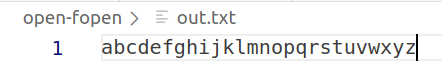
\includegraphics[width=150mm]{img/prog3_open.png}
	\caption{Результаты работы программы 3 (open и O\_APPEND)}
	\label{fig:prog-3-open-th-result}
\end{figure}






